\documentclass[a4paper, final]{article}
%\usepackage{literat} % Нормальные шрифты
\usepackage[14pt]{extsizes} % для того чтобы задать нестандартный 14-ый размер шрифта
\usepackage[T2A]{fontenc}
\usepackage[UTF8]{inputenc}
\usepackage[russian]{babel}
\usepackage{cmap}
\usepackage{listings} %листинги
\usepackage{amsmath}
\usepackage{amssymb} % Для красивого значка пустого множества
\usepackage[left=25mm, top=20mm, right=20mm, bottom=20mm, footskip=10mm]{geometry}
\usepackage{ragged2e} %для растягивания по ширине
\usepackage{setspace} %для межстрочного интервала
\usepackage{indentfirst} % для абзацного отступа
\usepackage{moreverb} %для печати в листинге исходного кода программ
\renewcommand\verbatimtabsize{4\relax}
\renewcommand\listingoffset{0.2em} %отступ от номеров строк в листинге
\renewcommand{\arraystretch}{1.4} % изменяю высоту строки в таблице
\usepackage[font=small, singlelinecheck=false, justification=centering, format=plain, labelsep=period]{caption} %для настройки заголовка таблицы
\usepackage{listingsutf8}
\usepackage{xcolor} % цвета
\usepackage{hyperref}% для гиперссылок
\usepackage{enumitem} %для перечислений
\usepackage{titlesec}
\usepackage{graphicx}
\graphicspath{ {./Рисунки/} }
%\usepackage{float}
\usepackage{booktabs}
\usepackage{floatrow}
\usepackage{scalerel} % Stretching images
\usepackage[final]{pdfpages}
\usepackage{multirow}
\usepackage{array}
\usepackage{tabularx}

\definecolor{apricot}{HTML}{FFF0DA}
\definecolor{mygreen}{rgb}{0,0.6,0}
\definecolor{string}{HTML}{B40000} % цвет строк в коде
\definecolor{comment}{HTML}{008000} % цвет комментариев в коде
\definecolor{keyword}{HTML}{1A00FF} % цвет ключевых слов в коде
\definecolor{morecomment}{HTML}{8000FF} % цвет include и других элементов в коде
\definecolor{captiontext}{HTML}{FFFFFF} % цвет текста заголовка в коде
\definecolor{captionbk}{HTML}{999999} % цвет фона заголовка в коде
\definecolor{bk}{HTML}{FFFFFF} % цвет фона в коде
\definecolor{frame}{HTML}{999999} % цвет рамки в коде
\definecolor{brackets}{HTML}{B40000} % цвет скобок в коде





\AtBeginDocument{\renewcommand{\contentsname}{Содержание}}
\AtBeginDocument{\renewcommand{\refname}{Список источников}}
% Настраиваем листинги, чтобы они использовали счётчик figure
\AtBeginDocument{
  \renewcommand{\thelstlisting}{\thefigure}  % Листинги используют тот же счетчик, что и рисунки
  \renewcommand{\lstlistingname}{Рис.}    % Меняем подпись
}

% Автоматически увеличиваем счетчик figure перед каждым листингом
\let\oldlstlisting\lstlisting
\renewcommand{\lstlisting}[1][]{%
    \refstepcounter{figure}% Увеличиваем счетчик figure
    \oldlstlisting[#1]% Вызываем оригинальную команду lstlisting
}
\lstset{
    captionpos=b
}
\newcommand{\specialcell}[2][l]{\begin{tabular}[#1]{@{}l@{}}#2\end{tabular}} % Алиас для таблиц

\floatsetup[table]{style=plain,capposition=top} % Подпись таблицы сверху
\setlist[enumerate,itemize]{leftmargin=1.2cm} %отступ в перечислениях

\hypersetup{colorlinks,
  allcolors=[RGB]{010 090 200}} %красивые гиперссылки (не красные)

% подгружаемые языки — подробнее в документации listings (это всё для листингов)
\lstloadlanguages{ [LaTeX] TeX}
% включаем кириллицу и добавляем кое-какие опции
\lstset{language =[LaTeX] TeX, % выбираем язык по умолчанию
extendedchars=true , % включаем не латиницу
escapechar = | , % |«выпадаем» в LATEX|
frame=tb , % рамка сверху и снизу
commentstyle=\itshape , % шрифт для комментариев
stringstyle =\bfseries} % шрифт для строк

\textheight=24cm % высота текста
\textwidth=16cm % ширина текста
\oddsidemargin=0pt % отступ от левого края
\topmargin=-1.5cm % отступ от верхнего края
\parindent=24pt % абзацный отступ
\parskip=0pt % интервал между абзацами
\tolerance=2000 % терпимость к "жидким" строкам
\flushbottom % выравнивание высоты страниц

\begin{document} % начало документа
\setcounter{tocdepth}{2} % Вложенность не больше 2 в содержании
\lstset{
  language=C++, % Язык кода по умолчанию
  escapeinside={(*@}{@*)}, % Позволяет использовать LaTeX-команды внутри кода
  morekeywords={*,...}, % если хотите добавить ключевые слова, то добавляйте
  % Цвета
  keywordstyle=\color{keyword}\ttfamily\bfseries,
  %stringstyle=\color{string}\ttfamily,
  stringstyle=\ttfamily\color{red!50!brown},
  commentstyle=\color{comment}\ttfamily,
  morecomment=[l][\color{morecomment}]{\#},
  % Настройки отображения
  breaklines=true, % Перенос длинных строк
  basicstyle=\ttfamily\footnotesize, % Шрифт для отображения кода
  backgroundcolor=\color{bk}, % Цвет фона кода
  frame=single,xleftmargin=\fboxsep,xrightmargin=-\fboxsep, % Рамка, подогнанная к заголовку
  rulecolor=\color{frame}, % Цвет рамки
  tabsize=3, % Размер табуляции в пробелах
  % Настройка отображения номеров строк. Если не нужно, то удалите весь блок
  numbers=left, % Слева отображаются номера строк
  stepnumber=1, % Каждую строку нумеровать
  numbersep=5pt, % Отступ от кода
  numberstyle=\small\color{black}, % Стиль написания номеров строк
  % Для отображения русского языка
  extendedchars=true,
  literate={Ö}{ {\"O} }1
  {~}{ {\textasciitilde} }1
  {а}{ {\selectfont\char224} }1
  {б}{ {\selectfont\char225} }1
  {в}{ {\selectfont\char226} }1
  {г}{ {\selectfont\char227} }1
  {д}{ {\selectfont\char228} }1
  {е}{ {\selectfont\char229} }1
  {ё}{ {\"e} }1
  {ж}{ {\selectfont\char230} }1
  {з}{ {\selectfont\char231} }1
  {и}{ {\selectfont\char232} }1
  {й}{ {\selectfont\char233} }1
  {к}{ {\selectfont\char234} }1
  {л}{ {\selectfont\char235} }1
  {м}{ {\selectfont\char236} }1
  {н}{ {\selectfont\char237} }1
  {о}{ {\selectfont\char238} }1
  {п}{ {\selectfont\char239} }1
  {р}{ {\selectfont\char240} }1
  {с}{ {\selectfont\char241} }1
  {т}{ {\selectfont\char242} }1
  {у}{ {\selectfont\char243} }1
  {ф}{ {\selectfont\char244} }1
  {х}{ {\selectfont\char245} }1
  {ц}{ {\selectfont\char246} }1
  {ч}{ {\selectfont\char247} }1
  {ш}{ {\selectfont\char248} }1
  {щ}{ {\selectfont\char249} }1
  {ъ}{ {\selectfont\char250} }1
  {ы}{ {\selectfont\char251} }1
  {ь}{ {\selectfont\char252} }1
  {э}{ {\selectfont\char253} }1
  {ю}{ {\selectfont\char254} }1
  {я}{ {\selectfont\char255} }1
  {А}{ {\selectfont\char192} }1
  {Б}{ {\selectfont\char193} }1
  {В}{ {\selectfont\char194} }1
  {Г}{ {\selectfont\char195} }1
  {Д}{ {\selectfont\char196} }1
  {Е}{ {\selectfont\char197} }1
  {Ё}{ {\"E} }1
  {Ж}{ {\selectfont\char198} }1
  {З}{ {\selectfont\char199} }1
  {И}{ {\selectfont\char200} }1
  {Й}{ {\selectfont\char201} }1
  {К}{ {\selectfont\char202} }1
  {Л}{ {\selectfont\char203} }1
  {М}{ {\selectfont\char204} }1
  {Н}{ {\selectfont\char205} }1
  {О}{ {\selectfont\char206} }1
  {П}{ {\selectfont\char207} }1
  {Р}{ {\selectfont\char208} }1
  {С}{ {\selectfont\char209} }1
  {Т}{ {\selectfont\char210} }1
  {У}{ {\selectfont\char211} }1
  {Ф}{ {\selectfont\char212} }1
  {Х}{ {\selectfont\char213} }1
  {Ц}{ {\selectfont\char214} }1
  {Ч}{ {\selectfont\char215} }1
  {Ш}{ {\selectfont\char216} }1
  {Щ}{ {\selectfont\char217} }1
  {Ъ}{ {\selectfont\char218} }1
  {Ы}{ {\selectfont\char219} }1
  {Ь}{ {\selectfont\char220} }1
  {Э}{ {\selectfont\char221} }1
  {Ю}{ {\selectfont\char222} }1
  {Я}{ {\selectfont\char223} }1
  {\{}{ { {\color{brackets}\{} } }1 % Цвет скобок {
  {\} }{ { {\color{brackets}\} } } }1 % Цвет скобок }
}

% НАЧАЛО ТИТУЛЬНОГО ЛИСТА
\begin{center}
\hfill \break
\hfill \break
\normalsize{МИНИСТЕРСТВО НАУКИ И ВЫСШЕГО ОБРАЗОВАНИЯ РОССИЙСКОЙ ФЕДЕРАЦИИ\\
 федеральное государственное автономное образовательное учреждение высшего образования «Санкт-Петербургский политехнический университет Петра Великого»\\[5pt]}
\normalsize{Институт компьютерных наук и кибербезопасности}\\[5pt] 
\normalsize{Высшая школа технологий искусственного интеллекта}\\[5pt] 
\normalsize{Направление: 02.03.01 Математика и компьютерные науки}\\

\hfill \break
\hfill \break
\hfill \break
\large{\textbf{Теория алгоритмов}}\\
\large{Отчёт по лабораторной работе №1}\\
\large{<<Реализация и анализ клеточного автомата>>}\\
\large{\textit{вариант 11\\}}

\hfill \break
\hfill \break
\end{center}
 
\small{ 
\begin{tabular}{lrrl}
\!\!\!Студент, & \hspace{2cm} & & \\
\!\!\!группы 5130201/20102 & \hspace{2cm} & \underline{\hspace{3cm}} & Гаар В.С. \\\\
\!\!\!Преподаватель & \hspace{2cm} & \underline{\hspace{3cm}} &  Востров А.В. \\\\
&&\hspace{5cm}
\end{tabular}
\begin{flushright}
<<\underline{\hspace{1cm}}>>\underline{\hspace{2.5cm}} 2024 г.
\end{flushright}
}

\hfill \break
\hfill \break
\hfill \break
\hfill \break
\hfill \break
\begin{center} \small{Санкт-Петербург, 2024} \end{center}
\thispagestyle{empty} % выключаем отображение номера для этой страницы

% КОНЕЦ ТИТУЛЬНОГО ЛИСТА
\newpage

\tableofcontents

\newpage

\cleardoublepage
\phantomsection
\addcontentsline{toc}{section}{Введение}
\section*{Введение}
Данный отчёт содержит в себе описание реализации лабораторной работы №1 по дисциплине <<Теория
алгоритмов>>, направленной на изучение аспектов работы клеточных автоматов. Содержание лабораторной
работы представлено ниже:
\begin{enumerate}
  \item Реализовать двумерный клеточный автомат с окрестностью фон Неймана в соответствии с 
  полученным номером № = $2424840_{10}$.
  \item Реализовать торроидальные, нулевые, единичные граничные условия с возможностью выбора пользователем.
  \item Пользователь определяет ширину поля и количество итераций. 
  \item Необходимо учесть возможность ввода различных начальных условий (как вручную, так и 
  случайным образом) по выбору пользователя. 
  \item Отображение реализовать в консоли.
  \item Проанализировать свой клеточный автомат в отчете (его поведение, паттерны, <<сходимость>> 
  и т.д.). 
\end{enumerate}

\newpage
\section{Математическое описание}
\subsection{Клеточные автоматы}
\textbf{Клеточный автомат} представляет собой двусторонне бесконечную ленту, каждая ячейка 
которой может находиться в некотором состоянии. Множество состояний $Q$, обозначим состояние ячейки $i$ 
как $s[i]$. Изначально все ячейки находятся в состоянии $B \in Q$, кроме ячеек с номерами от $1$ до $n$. 
Ячейка с номером $i$, где $1 \leq i \leq n$ находится в состоянии $x_i$, где $x$ -- входное слово
(будем считать, что $\Sigma \subset Q, B \not \in \Sigma$).


Правила работы клеточного автомата такие: задано число $d$ и функция $f: Q^{2d+1} \rightarrow Q$. 
За один шаг все клетки меняют состояние по следующему правилу: новое состояние клетки $i$ равно 
$f(s[i-d],s[i-d+1],\dots,s[i+d-1],s[i+d])$. Если клетка с номером 0 переходит в состояние $Y$, 
то автомат допускает слово $x$.

\textbf{Клеточным автоматом} (КА) (англ. \textit{cellular automaton}) $A$ размерности $d$ 
называется четверка $<Z^d,S,N,\delta>$, где
\begin{itemize}
\item $S$ -- конечное множество, элементы которого являются состояниями $A$.
\item $N$ -- конечное упорядоченное подмножество $Z^d$, $N=\{n_j | n_j = (x_{1_j},\dots,x_{d_j}),
j \in \{1 \dots n\}\}$, называемое \textbf{окрестностью} (англ. \textit{neighborhood}) $A$.
В данном определении полагается, что клетка всегда принадлежит своей окрестности.
\item $\delta : S_n \rightarrow S$ -- функция перехода для $A$. \cite{bib:linearcellularautomaton}
\end{itemize}

\textbf{Окрестность фон Неймана} ячейки --- совокупность ячеек в сетке 
(двумерном паркете, трёхмерном Евклидовом пространстве, разбитом на равновеликие кубы), 
имеющих общую сторону (грань) с данной ячейкой. \cite{bib:cellularautomaton}

Пример двумерной окрестности фон Неймана порядка 1 представлен на рисунке №~\ref{img:neyman}.
\begin{figure}[H]
   \centering
   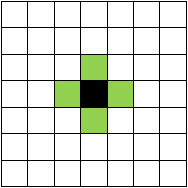
\includegraphics[scale=1]{neyman.png}
   \caption{Двумерная окрестность фон Неймана порядка 1}
   \label{img:neyman}
\end{figure}

\textbf{Двумерный клеточный автомат} можно определить как множество конечных автоматов на плоскости, 
помеченных целочисленными координатами $(i, j)$, каждый из которых может находиться в одном из состояний
$$\sigma _{i,j}: \sigma _{i,j}\in \Sigma \equiv \{0,1,2...k-1,k\}, \quad i, j \in \mathbb{N} \cup \{0\}.$$

\noindent Изменение состояний автоматов происходит согласно правилу перехода
$$ \sigma _{i,j}(t+1)=\phi (\sigma _{k,l}(t)|(k,l)\in {\mathcal {N}}(i,j)), \quad i, j \in \mathbb{N} \cup \{0\},$$

\noindent где ${\mathcal {N}}(i,j)$ -- некоторая окрестность точки $(i,j)$. 
К примеру, окрестность фон Неймана определяется как 
$${\mathcal {N}}_{N}^{1}(i,j)=\{(k,l):~|i-k|+|j-l|\leq 1\}, \quad i, j \in \mathbb{N} \cup \{0\},$$
\noindent а окрестность Мура
$$\displaystyle {\mathcal {N}}_{M}^{1}(i,j)=\{(k,l):~|i-k|\leq 1,|j-l|\leq 1\},  \quad i, j \in \mathbb{N} \cup \{0\}.$$

Число всех возможных правил перехода определяется числом состояний 
$\sigma$ и количеством соседей $n$ и составляет 
$$N_{r}=\sigma ^{\sigma ^{n}}\cite{bib:2dcellularautomaton}$$ 

Граничные условия Определяют, как будет выглядеть окрестность клеток на границах сетки. Основные типы:
\begin{itemize}
    \item \textit{Нулевые граничные условия:} За пределами сетки клетки считаются находящимися в нулевом состоянии.
    \[
        S(i, j) = 
        \begin{cases} 
            0, & \text{если } i < 0 \text{ или } i \geq N \text{ или } j < 0 \text{ или } j \geq M, \\
            C(i, j), & \text{иначе},
        \end{cases}
        \]
    \item \textit{Единичные граничные условия:} За пределами сетки клетки считаются находящимися в единичном состоянии.
    \[
        S(i, j) = 
        \begin{cases} 
            1, & \text{если } i < 0 \text{ или } i \geq N \text{ или } j < 0 \text{ или } j \geq M, \\
            C(i, j), & \text{иначе},
        \end{cases}
        \]
    \item \textit{Тороидальные граничные условия:} Сетка рассматривается как тор, то есть клетки на одной границе соединены с противоположной границей.
    \[
        S(i, j) = 
        \begin{cases} 
            C((i + N)\!\!\!\! \mod N, (j + M)\!\!\!\! \mod M), & \text{если } i < 0 \text{ или } i \geq N \\
            & \quad \text{или } j < 0 \text{ или } j \geq M, \\
            C(i, j), & \text{иначе},
        \end{cases}
    \]    
\end{itemize}

где \(N\) и \(M\) — размеры сетки.

\subsection{Классификация клеточных автоматов}
\subsubsection{Классификация по типам поведения}
Стивен Вольфрам в своей книге A New Kind of Science предложил 4 класса, на которые 
все клеточные автоматы могут быть разделены в зависимости от типа их эволюции. 
Классификация Вольфрама была первой попыткой классифицировать сами правила, а не типы 
поведения правил по отдельности. В порядке возрастания сложности классы выглядят следующим 
образом:
\begin{itemize}
\item Класс 1: Результатом эволюции начальных условий является быстрый переход к гомогенной стабильности. Любые негомогенные конструкции быстро исчезают.
\item Класс 2: Результатом эволюции начальных условий является быстрый переход в неизменяемое негомогенное состояние либо возникновение циклической последовательности. Большинство структур начальных условий быстро исчезает, но некоторые остаются. Локальные изменения в начальных условиях оказывают локальный характер на дальнейший ход эволюции системы.
\item Класс 3: Результатом эволюции почти всех начальных условий являются псевдо-случайные, хаотические последовательности. Любые стабильные структуры, которые возникают почти сразу же уничтожаются окружающим их шумом. Локальные изменения в начальных условиях оказывают неопределяемое влияние на ход эволюции системы.
\item Класс 4: Результатом эволюции являются структуры, которые взаимодействуют сложным образом с формированием локальных, устойчивых структур. В результате эволюции могут получаться некоторые последовательности Класса 2, описанного выше. Локальные изменения в начальных условиях оказывают неопределяемое влияние на ход эволюции системы. Некоторые клеточные автоматы этого класса обладают свойством универсальности по Тьюрингу, что доказано для Правила 110 и игры «Жизнь».
\end{itemize}


\subsection{Тоталистичные клеточные автоматы}
Существует специальный класс клеточных автоматов, называемых тоталистичными. 
На каждом шаге эволюции клеточного автомата значение клетки равно какому-либо целому числу
(обычно выбираемого из конечного множества), а новое состояние клетки определяется суммой 
 значений клеток-соседей и, возможно, предыдущим состоянием клетки. Если состояние клетки на 
 новом шаге зависит от её предыдущего состояния, то такой клеточный автомат называется внешним 
 тоталистичным. Игра Жизнь является примером внешнего тоталистического клеточного автомата с 
 набором значений ячеек $0,1$.  

Термин тоталистичный происходит от английского \textit{totalistic}. В свою очередь 
\textit{total} может быть переведено как сумма, что и отражено в принципе действия этого 
типа автоматов, когда новое значение клетки зависит от суммы значений других клеток.

\subsection{Представление функции с данным №}
Номер функции был вычислен по следующему выражению: № = номер варианта * 11 * год рождения * день * месяц,
где номер варианта = 11. Получилось значение $2424840_{10}$, которое далее было представлено в двоичном
виде и дополнено до 32 символов незначащими ведущими нулями. Далее использовался  получившийся 
вектор-столбец 
$$f(s_0, s_1, s_2, s_3, s_4) = (00000000001001010000000000001000)_2,$$
\noindent где переменные $s_0, s_1, s_2, s_3, s_4$ соответствуют следующим клеткам в окрестности 
фон Неймана, представленным на рисунке №~\ref{img:neyman_vars}:
\begin{figure}[H]
   \centering
   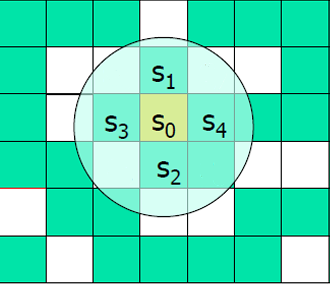
\includegraphics[scale=1]{neyman_vars.png}
   \caption{Нумерация клеток в окрестности фон Неймана}
   \label{img:neyman_vars}
\end{figure}

\newpage
\section{Особенности реализации}
Сам двумерный клеточный автомат реализован в виде класса \texttt{CellularAutomaton} со следующими
характеристиками:
\begin{itemize}
  \item \textbf{Поля}:
  \begin{itemize}
    \item \texttt{std::mt19937 rng}: переменная, используемая для генерации случайных чисел;
    \item \texttt{int width, height}: переменные для хранения ширины и высоты поля соответственно;
    \item \texttt{std::string rule}: переменная, используемая для хранения вектора-столбца значений
    двоичной функции $f(s_0, s_1, s_2, s_3, s_4)$ в виде строки;
    \item \texttt{std::string boundaryCondition}: переменная для хранения формата граничных условий -
    <<zero>>, <<one>>, <<toroidal>>;
    \item \texttt{std::vector<std::vector<int>> field}: контейнер для хранения текущего состояния
    клеточного поля;
    \item \texttt{std::vector<std::vector<int>> nextField}: контейнер для хранения следующего
    состояния клеточного поля, сдвинутого на один такт эволюции вперёд.
  \end{itemize}
  
  \item \textbf{Методы}:
  \begin{itemize}
    \item \texttt{void evolve()}: метод, выполняющий сдвиг клеточного поля на один такт эволюции
    вперёд;
    \item \texttt{void display() const}: метод для отображения текущего состояния клеточного поля
    на консоль;
    \item \texttt{void setInitialState()}: метод для задания исходного состояния клеточного поля
    пользователем;
    \item \texttt{void generateInitialState()}: private-метод для случайной генерации исходного 
    состояния клеточного поля;
    \item \texttt{unsigned int countAliveNeighbors(int x, int y) const}: private-метод для подсчёта
    количества <<живых>> клеток, граничащих с клеткой с координатами $(x,  y)$;
    \item \texttt{int getCell(int x, int y) const}: метод для получения значения клетки, расположенной
    по координатам $(x, y)$ с учётом заданных граничных условий в поле boundaryCondition.
  \end{itemize}
\end{itemize}

Код создания данного класса приведён на рисунке №~\ref{lst:class}.

\begin{lstlisting}[caption={Код создания класса \texttt{CellularAutomaton}}, 
  label={lst:class}]
class CellularAutomaton
{
    std::mt19937 rng;

    int width, height;
    std::string rule;
    std::string boundaryCondition;
    std::vector<std::vector<int>> field;
    std::vector<std::vector<int>> nextField;

public:
    CellularAutomaton(int width, int height, std::string rule, std::string boundaryCondition, bool randomInit = false);

    void evolve();

    void display() const;

    void setInitialState();
    
private:
    void generateInitialState();

    unsigned int countAliveNeighbors(int x, int y) const;

    int getCell(int x, int y) const;
};  
\end{lstlisting}

\subsection{Функция получения значения клетки}
Функция принимает на вход два параметра -- координаты клетки $(x, y)$, значение которой Необходимо
получить. Далее функция обрабатывает каждый из возможных вариантов граничных условий в поле 
\texttt{boundaryCondition} и возвращает соответствующее значение. Код реализации метода \texttt{getCell}
представлен на рисунке №~\ref{lst:getCell}.

\begin{verbatim}
  Вход: координаты клетки x, y типа int.
  
  Выход: значение клетки поля типа int в соответствии с её координатами и 
  заданным граничным условием.
\end{verbatim}

\begin{lstlisting}[caption={Код реализации метода \texttt{getCell}}, label={lst:getCell}]
int CellularAutomaton::getCell(int x, int y) const {
  if (boundaryCondition == "toroidal") {
    if (x < 0) {
      return field[height - 1][y];
    }
    else if(x > height) {
      return field[0][y];
    }

    if (y < 0) {
      return field[x][width-1];
    }
    else if (y > width) {
      return field[x][0];
    }
    return field[x%height][y%width];
  }
  else if (boundaryCondition == "zero") {
    if (x < 0 || x >= height || y < 0 || y >= width) {
      return 0;
    }
    return field[x][y];
  }
  else if (boundaryCondition == "one") {
    if (x < 0 || x >= height || y < 0 || y >= width) {
      return 1;
    }
    return field[x][y];
  }
  return 0;
}
\end{lstlisting}

\subsection{Функция подсчёта количества живых клеток}
Функция \texttt{countAliveNeighbors} подсчитывает состояния соседей клетки, используя метод \texttt{getCell} 
для получения их значений. Возвращает закодированное целое число, где состояния соседей закодированы битами.
Каждый сосед представлен в виде отдельного бита:
\begin{itemize}
  \item Сосед сверху $s_1$ -- 8-й бит (самый старший, s1 << 3).
  \item Сосед снизу $s_2$ -- 4-й бит.
  \item Сосед слева $s_3$ -- 2-й бит.
  \item Сосед справа $s_4$ -- 1-й бит (самый младший, s4).
\end{itemize}

Код реализации метода \texttt{countAliveNeighbors} представлен на рисунке №~\ref{lst:countAliveNeighbors}.

\begin{verbatim}
Вход:
x (тип int): координата клетки по оси X.
y (тип int): координата клетки по оси Y.

Выход:
Возвращает unsigned int: целое число, где состояния соседей закодированы в
4 битах.
\end{verbatim}

\begin{lstlisting}[caption={Код реализации метода \texttt{countAliveNeighbors}}, label={lst:countAliveNeighbors}]
unsigned int CellularAutomaton::countAliveNeighbors(int x, int y) const {
  unsigned int s1 = getCell(x, y - 1);
  unsigned int s2 = getCell(x, y + 1);
  unsigned int s3 = getCell(x - 1, y);
  unsigned int s4 = getCell(x + 1, y);

  return (s1 << 3) + (s2 << 2) + (s3 << 1) + s4;
}
\end{lstlisting}

\subsection{Функция перехода к следующему состоянию}
Функция \texttt{evolve} вычисляет следующее состояние клеточного автомата. Она проходит через каждую клетку, 
подсчитывает состояния соседей, используя \texttt{countAliveNeighbors}, определяет новое состояние клетки на 
основе текущего состояния и правила, закодированного в строке \texttt{rule}, и сохраняет новое состояние в массиве 
\texttt{nextField}. Затем обновляет основное поле \texttt{field} значениями из \texttt{nextField}.

Код реализации метода \texttt{evolve} представлен на рисунке №~\ref{lst:evolve}.

\begin{verbatim}
Вход:
field (тип std::vector<std::vector<int>>)
Текущее состояние клеточного автомата, представленное в виде двумерного 
массива.

width (тип int)
Ширина поля (количество столбцов).

height (тип int)
Высота поля (количество строк).

rule (тип std::string)
Правило перехода клеточного автомата, закодированное в строке.

nextField (тип std::vector<std::vector<int>>)
Временный массив для записи новых состояний клеток.

Выход:
Поле field обновляется до следующего поколения.
\end{verbatim}

\begin{lstlisting}[caption={Код реализации метода \texttt{evolve}}, label={lst:evolve}]
void CellularAutomaton::evolve() {
  // Проходим по каждой клетке
  for (int x = 0; x < height; x++) {
    for (int y = 0; y < width; y++) {
      // Подсчитываем количество живых соседей для клетки (x, y)
      int aliveNeighbors = countAliveNeighbors(x, y);

      // Текущий статус клетки
      int currentState = field[x][y];

      // Вычисляем индекс в правиле для данной клетки и соседей
      int ruleIndex = (currentState << 4) | aliveNeighbors;
      int newState = (rule[ruleIndex] == '1') ? 1 : 0;

      // Обновляем nextField для данной клетки
      nextField[x][y] = newState;
    }
  }

  // Копируем nextField в field для следующего поколения
  for (int x = 0; x < height; x++) {
    for (int y = 0; y < width; y++) {
      field[x][y] = nextField[x][y];
    }
  }
}
\end{lstlisting}
  

\newpage
\section{Результаты работы программы}
На рисунке №~\ref{img:example1} представлено создание клеточного автомата №1 с полем 2x2, ручным заданием начального
состояния, единичными границами и количеством итераций, равным 4.
\begin{figure}[H]
   \centering
   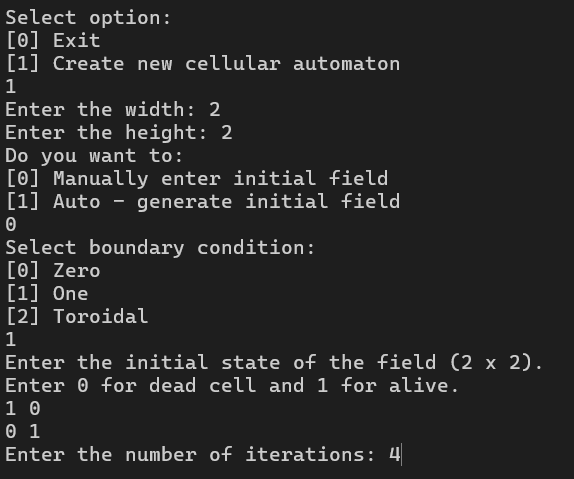
\includegraphics[scale=0.6]{example1.png}
   \caption{Создание клеточного автомата №1}
   \label{img:example1}
\end{figure}

На рисунке №~\ref{img:example1_res} представлены результаты эволюции клеточного автомата №1 за все 4 итерации.

\begin{figure}[H]
  \centering
  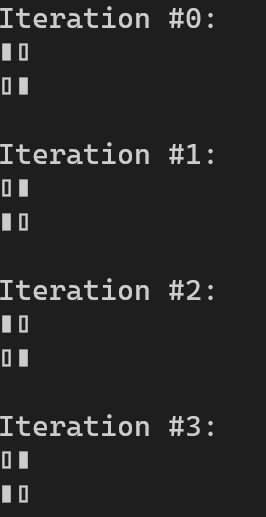
\includegraphics[scale=0.6]{example1_res.png}
  \caption{Итерации эволюции клеточного автомата №1}
  \label{img:example1_res}
\end{figure}


На рисунке №~\ref{img:example2} представлено создание клеточного автомата №2 с полем 2x2, ручным заданием начального
состояния, тороидальными границами и количеством итераций, равным 4.
\begin{figure}[H]
   \centering
   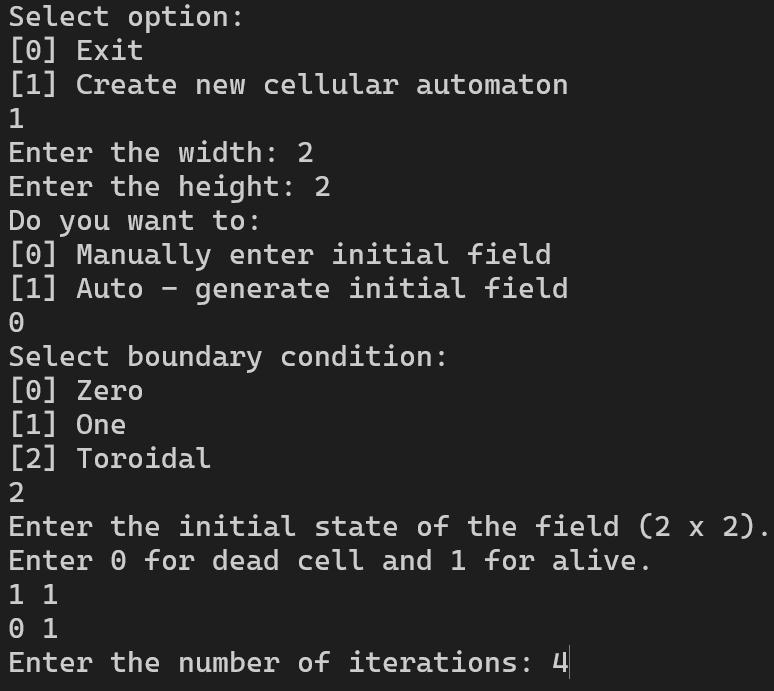
\includegraphics[scale=0.6]{example2.png}
   \caption{Создание клеточного автомата №2}
   \label{img:example2}
\end{figure}

На рисунке №~\ref{img:example2_res} представлены результаты эволюции клеточного автомата №2 за все 4 итерации.

\begin{figure}[H]
  \centering
  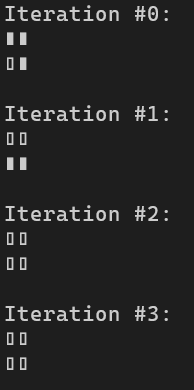
\includegraphics[scale=0.6]{example2_res.png}
  \caption{Итерации эволюции клеточного автомата №2}
  \label{img:example2_res}
\end{figure}

На рисунке №~\ref{img:example3} представлено создание клеточного автомата №3 с полем 20x20, автоматическим заданием 
начального состояния, нулевыми границами и количеством итераций, равным 4.
\begin{figure}[H]
   \centering
   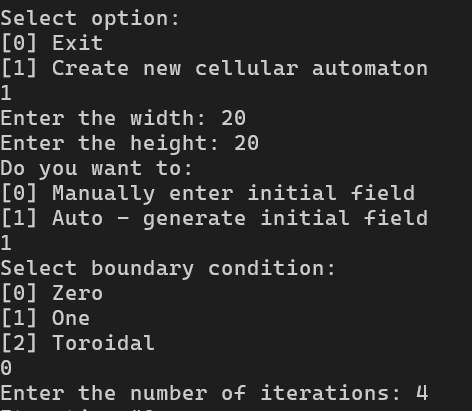
\includegraphics[scale=0.6]{example3.png}
   \caption{Создание клеточного автомата №3}
   \label{img:example3}
\end{figure}

На рисунке №~\ref{img:example3_res} представлены результаты эволюции клеточного автомата №3 за все 4 итерации.

\begin{figure}[H]
  \centering
  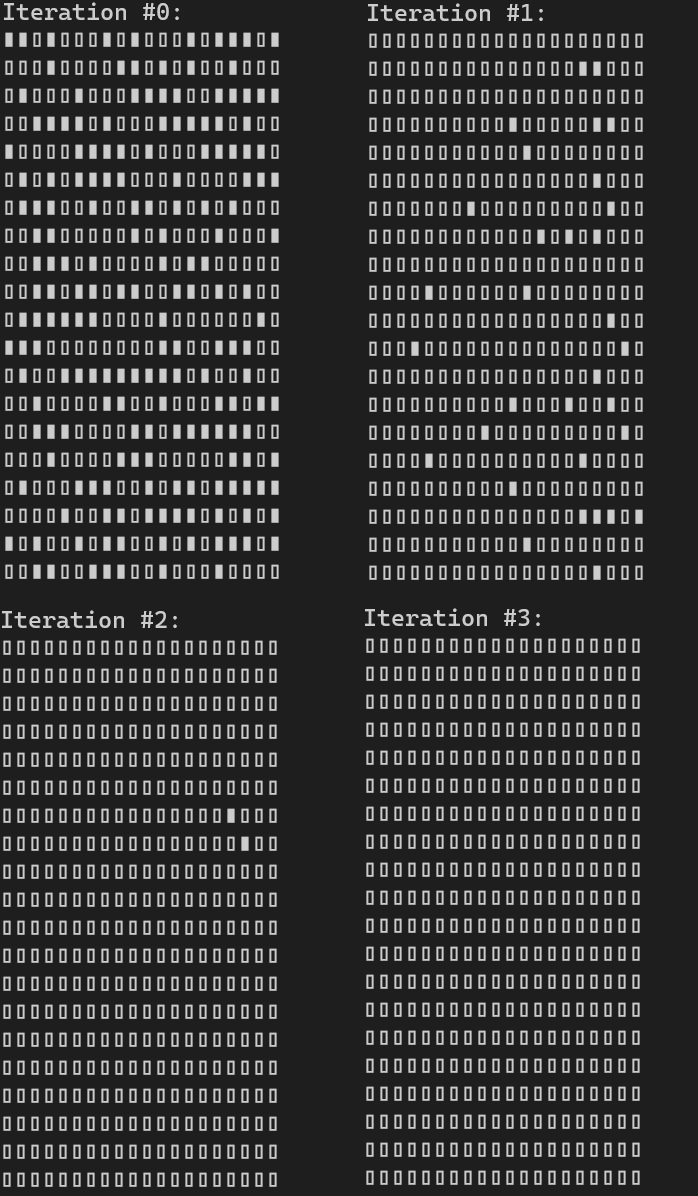
\includegraphics[scale=0.4]{example3_res.png}
  \caption{Итерации эволюции клеточного автомата №3}
  \label{img:example3_res}
\end{figure}

На рисунке №~\ref{img:example4} представлено создание клеточного автомата №4 с полем 5x5, автоматическим заданием 
начального состояния, единичными границами и количеством итераций, равным 20.
\begin{figure}[H]
   \centering
   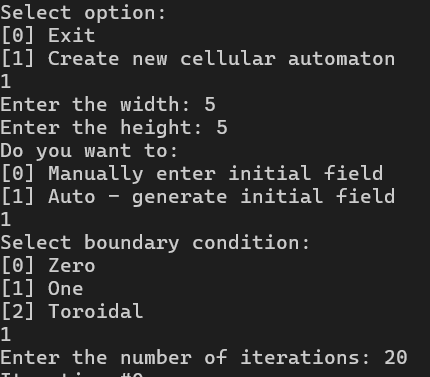
\includegraphics[scale=0.6]{example4.png}
   \caption{Создание клеточного автомата №4}
   \label{img:example4}
\end{figure}

На рисунке №~\ref{img:example4_res} представлены результаты эволюции клеточного автомата №4 за все 20 итераций.

\begin{figure}[H]
  \centering
  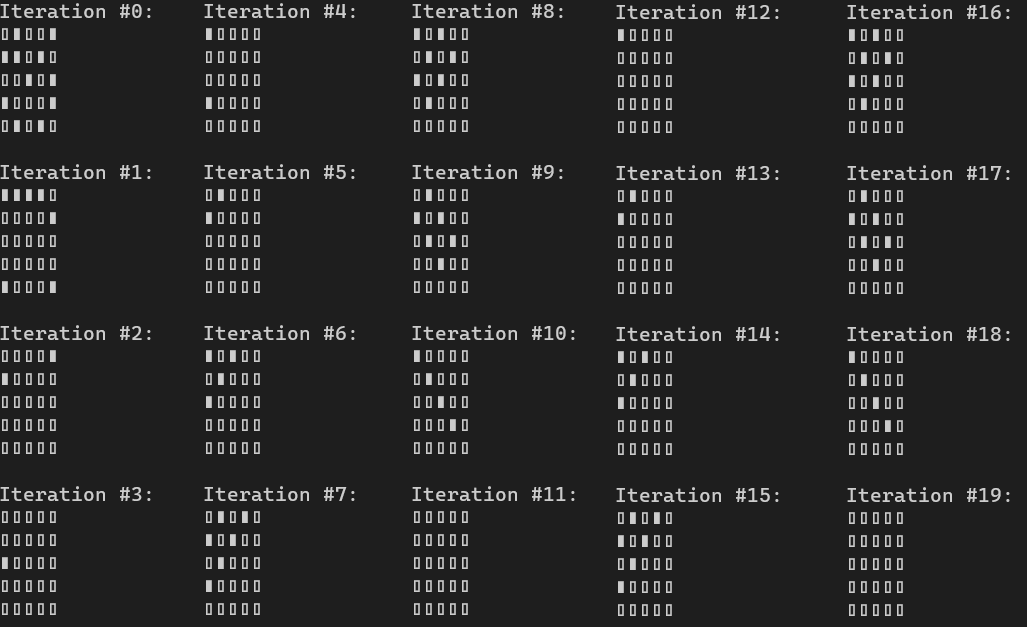
\includegraphics[scale=0.6]{example4_res.png}
  \caption{Итерации эволюции клеточного автомата №4}
  \label{img:example4_res}
\end{figure}

\newpage
\section{Анализ клеточного автомата}
В  итоге получился клеточный автомат, реализующий правило $2424840_{10}$ с четырьмя соседями (окрестность фон Неймана). 
Граничные условия выбирает пользователь (торроидальные, нулевые, единичные). Начальные состояния генерируются 
случайным образом или задаются пользователем. 

Для анализа использовались пять случайно сгенерированных полей размером 20x20.
Автомат эволюционирует, обновляя каждую клетку на основе правила, учитывающего текущее состояние и число 
активных соседей.

Реализованный клеточный автомат с единичными границами и любым начальным состоянием:
\begin{itemize}
  \item Демонстрирует периодический паттерн, устойчивый к изменениям начальных условий.
  \item Демонстрирует цикличность, которая возникает через 3–5 итераций (в зависимости от начального состояния).
  \item Полностью не затухает: количество живых клеток остаётся постоянным на каждом цикле.
  \item Появляется устойчивый рисунок в виде прямоугольника, перемещающегося из левого верхнего угла в правый нижний
  и постепенно уменьшающегося по высоте.
  \item Сходится к периодичности состояний (рис.~\ref{img:graph_one}, \ref{img:approx_one}).
  \item Относится к классу 2 по классификации Вольфрама.
  \item Напоминает биологические циклы, такие как суточные ритмы или процессы восстановления.
\end{itemize}

\begin{figure}[h!]
   \centering
   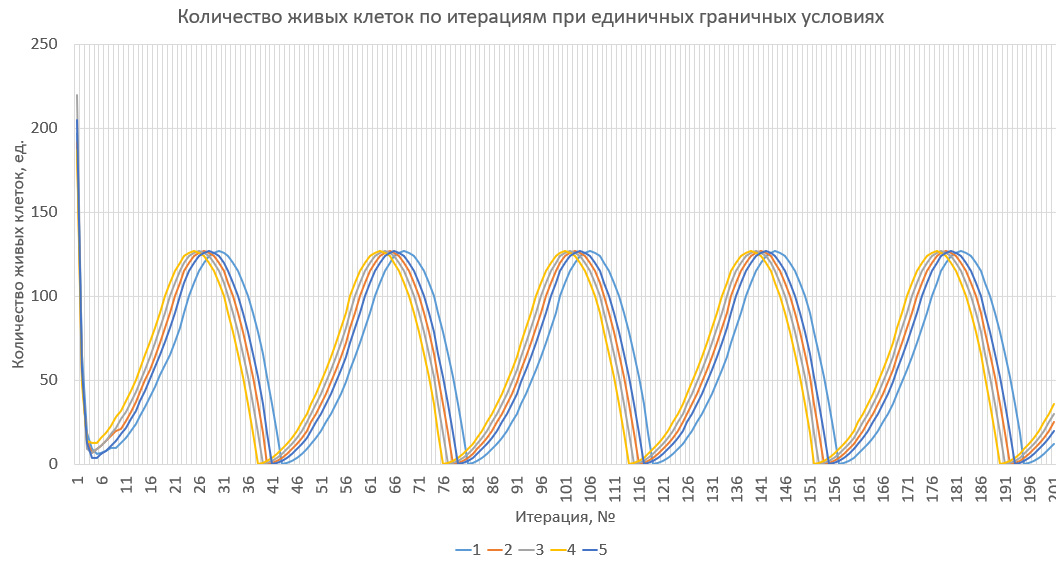
\includegraphics[width=0.8\linewidth]{graph_one.png}
   \caption{График количества живых клеток по итерациям при единичных граничных условиях}
   \label{img:graph_one}
\end{figure}

\begin{figure}[h!]
  \centering
  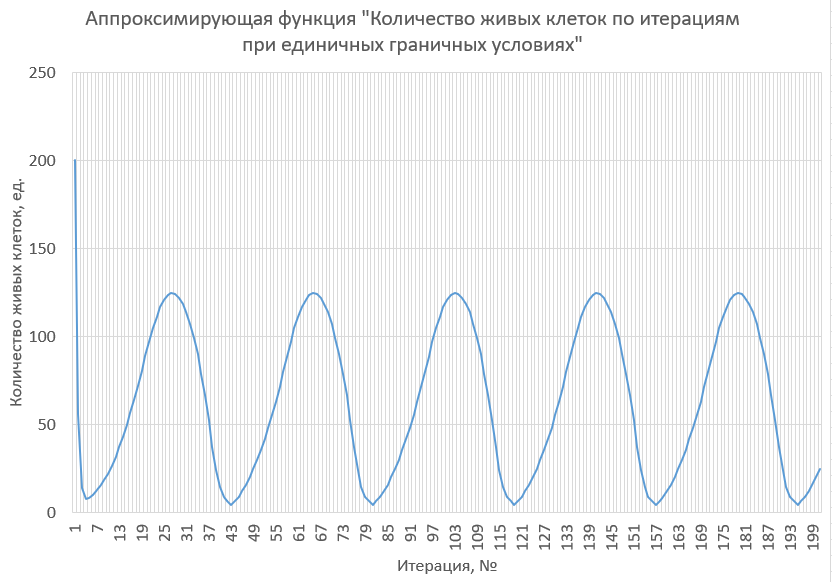
\includegraphics[width=0.8\linewidth]{approx_one.png}
  \caption{График аппроксимирующей функции количества живых клеток по итерациям при единичных граничных условиях}
  \label{img:approx_one}
\end{figure}

Реализованный клеточный автомат с нулевыми и тороидальными границами и любым начальным состоянием:
\begin{itemize}
  \item Демонстрирует хаотичный паттерн в первые 2–3 итерации.
  \item Полностью затухает к 3–4 итерации, независимо от начальных условий.
  \item Не демонстрирует устойчивых структур или цикличности.
  \item Отсутствуют локальные области порядка.
  \item Сходится к состоянию исчезновения всех живых клеток (рис.~\ref{img:graph_zero}-\ref{img:approx_toroidal}).
  \item Относится к классу 1 по классификации Вольфрама.
  \item Для полностью заполненного единичного поля автомат затухает быстрее -- за одну итерацию.
  \item Напоминает диссипативный процесс, например, рассеивание тепла или угасание волн.
\end{itemize}

\begin{figure}[h!]
  \centering
  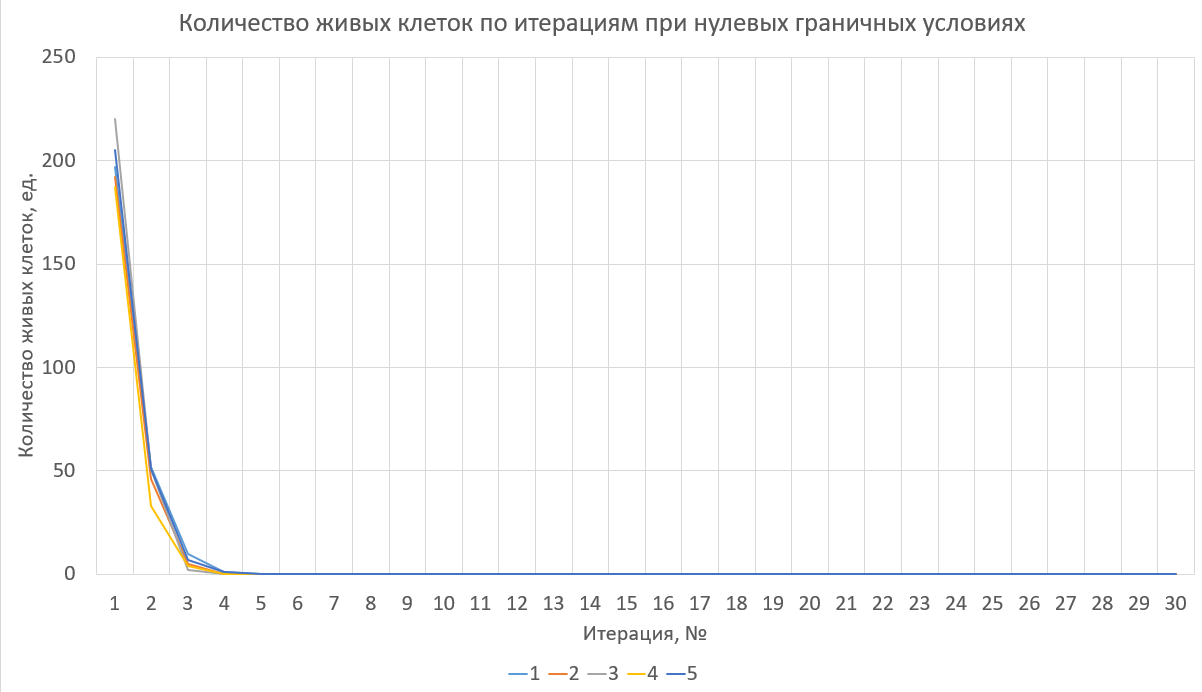
\includegraphics[width=0.8\linewidth]{graph_zero.png}
  \caption{График количества живых клеток по итерациям при нулевых граничных условиях}
  \label{img:graph_zero}
\end{figure}

\begin{figure}[h!]
 \centering
 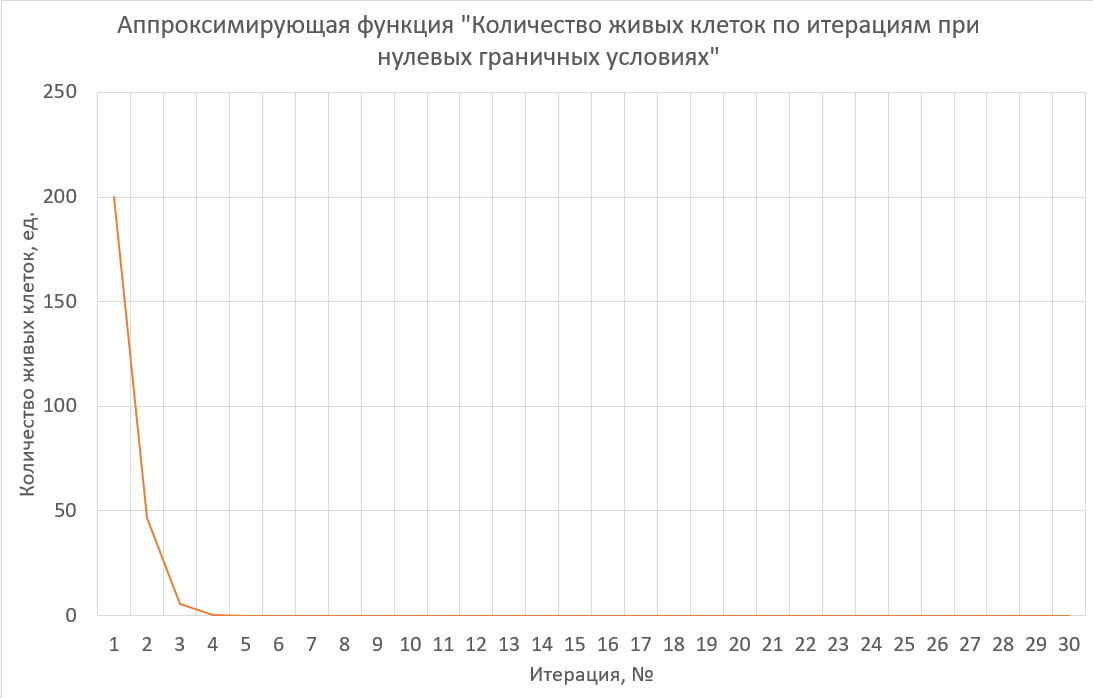
\includegraphics[width=0.8\linewidth]{approx_zero.png}
 \caption{График аппроксимирующей функции количества живых клеток по итерациям при нулевых граничных условиях}
 \label{img:approx_zero}
\end{figure}

\begin{figure}[h!]
  \centering
  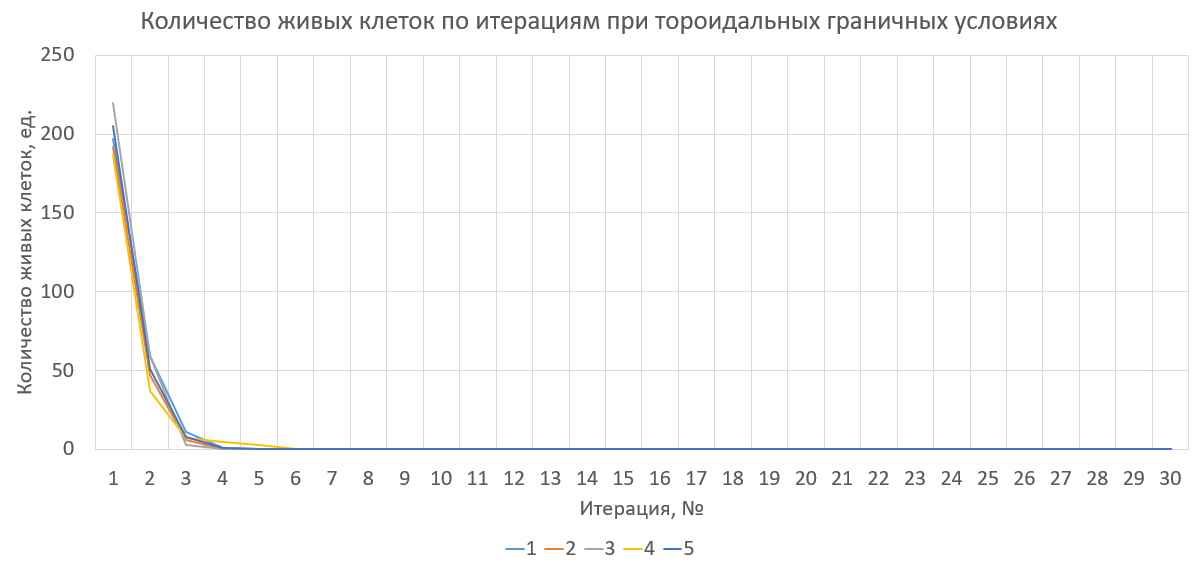
\includegraphics[width=0.8\linewidth]{graph_toroidal.png}
  \caption{График количества живых клеток по итерациям при тороидальных граничных условиях}
  \label{img:graph_toroidal}
\end{figure}

\begin{figure}[h!]
 \centering
 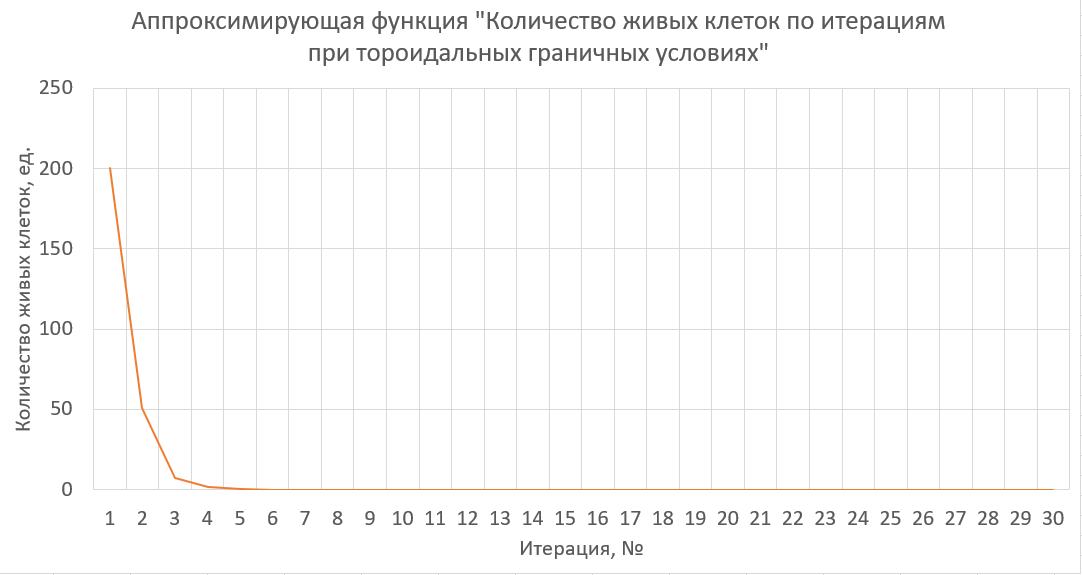
\includegraphics[width=0.8\linewidth]{approx_toroidal.png}
 \caption{График аппроксимирующей функции количества живых клеток по итерациям при тороидальных граничных условиях}
 \label{img:approx_toroidal}
\end{figure}

\cleardoublepage
\phantomsection
\newpage
\addcontentsline{toc}{section}{Заключение}
\section*{Заключение}
В ходе выполнения лабораторной работы №1 были выполнены следующие задачи:
\begin{enumerate}
  \item Реализован двумерный клеточный автомат с окрестностью фон Неймана в соответствии с 
  полученным номером № = $2424840_{10}$.
  \item Реализованы торроидальные, нулевые, единичные граничные условия с возможностью выбора пользователем.
  \item Пользователь определяет ширину поля и количество итераций. 
  \item Учтена возможность ввода различных начальных условий (как вручную, так и 
  случайным образом) по выбору пользователя. 
  \item Отображение было реализовано в консоли.
  \item Проанализирован клеточный автомат в отчете.
\end{enumerate}

\noindent Из достоинств реализации можно отметить:
\begin{itemize}
  \item Поддержка нескольких типов границ (торроидальные, нулевые, единичные).
  \item Обобщённость правила.
\end{itemize}

\noindent Из недостатков реализации можно отметить: 
\begin{itemize}
  \item Ограниченность правил: возможность задавать только одно фиксированное правило за запуск.
  \item Фиксированная окрестность: используется только окрестность фон Неймана.
  \item Отсутствие статистики.
  \item Ограниченная визуализация.
\end{itemize}

Проект располагает к масштабированию: имеется возможность добавить поддержку окрестности Мура, внедрить возможность
задания правила в виде 32-битного двоичного числа через пользовательский интерфейс, внедрить сбор статистики, добавить графическую визуализацию.

Работа была выполнена в среде разработки Microsoft Visual Studio 2022 (v143). Использовался стандарт языка ISO C++ 14 и
компилятор MSVC версии 14.32.31326. Была выбрана платформа решений x64.

Исходный код всего проекта находится в \href{https://github.com/vlgUseless/CellularAutomaton}
{репозитории GitHub} (\url{https://github.com/vlgUseless/CellularAutomaton}).

Полученные знания могут быть и будут испольованы в работе над последующими проектами и заданиями.
\cleardoublepage
\phantomsection
\newpage
%Список источников
\begin{thebibliography}{0}
  \bibitem{bib:linearcellularautomaton}
	ИТМО. Линейный клеточный автомат, эквивалентность МТ [Электронный ресурс] URL: 
  https://neerc.ifmo.ru/wiki/index.php?title=Линейный\_клеточный\_ \ автомат,\_эквивалентность\_МТ
  (дата обращения 20.11.2024).

	\bibitem{bib:cellularautomaton}
	ИТМО. Модели клеточных автоматов [Электронный ресурс] URL: 
  https://neerc.ifmo.ru/wiki/index.php?title=Модели\_клеточных\_автоматов 
  (дата обращения 20.11.2024).

  \bibitem{bib:2dcellularautomaton}
	A.G.Hoekstra, J.Kroc, P.Sloot. Simulating complex systems by cellular automata. Springer, 
  2010. ISBN 978-3-642-12202-6
\end{thebibliography}
\addcontentsline{toc}{section}{Список источников}

\end{document}